\documentclass[a4paper]{scrreprt}

% Uncomment to optimize for double-sided printing.
% \KOMAoptions{twoside}

% Set binding correction manually, if known.
% \KOMAoptions{BCOR=2cm}

% Localization options
\usepackage[english]{babel}
\usepackage[T1]{fontenc}
\usepackage[utf8]{inputenc}

% Quotations
\usepackage{dirtytalk}

% Floats
\usepackage{float}

\usepackage{numbertabbing}

% Enhanced verbatim sections. We're mainly interested in
% \verbatiminput though.
\usepackage{verbatim}

% Automatically remove leading whitespace in lstlisting
\usepackage{lstautogobble}

% PDF-compatible landscape mode.
% Makes PDF viewers show the page rotated by 90°.
\usepackage{pdflscape}

% Advanced tables
\usepackage{array}
\usepackage{tabularx}
\usepackage{longtable}

% Fancy tablerules
\usepackage{booktabs}

% Graphics
\usepackage{graphicx}

% Current time
\usepackage[useregional=numeric]{datetime2}

% Float barriers.
% Automatically add a FloatBarrier to each \section
\usepackage[section]{placeins}

% Custom header and footer
\usepackage{fancyhdr}

\usepackage{geometry}
\usepackage{layout}

% Math tools
\usepackage{mathtools}
% Math symbols
\usepackage{amsmath,amsfonts,amssymb}
\usepackage{amsthm}
% General symbols
\usepackage{stmaryrd}

% Utilities for quotations
\usepackage{csquotes}

% Bibliography
\usepackage[
  style=alphabetic,
  backend=biber, % Default backend, just listed for completness
  sorting=ynt % Sort by year, name, title
]{biblatex}
\addbibresource{references.bib}

\DeclarePairedDelimiter\abs{\lvert}{\rvert}
\DeclarePairedDelimiter\floor{\lfloor}{\rfloor}

% Bullet point
\newcommand{\tabitem}{~~\llap{\textbullet}~~}

\floatstyle{ruled}
\newfloat{algo}{htbp}{algo}
\floatname{algo}{Algorithm}
% For use in algorithms
\newcommand{\str}[1]{\textsc{#1}}
\newcommand{\var}[1]{\textit{#1}}
\newcommand{\op}[1]{\textsl{#1}}

\pagestyle{plain}
% \fancyhf{}
% \lhead{}
% \lfoot{}
% \rfoot{}
% 
% Source code & highlighting
\usepackage{listings}

% SI units
\usepackage[binary-units=true]{siunitx}
\DeclareSIUnit\cycles{cycles}

% Convenience commands
\newcommand{\mailsubject}{41106 - Cryptography Protocols - Series 8}
\newcommand{\maillink}[1]{\href{mailto:#1?subject=\mailsubject}
                               {#1}}

% Should use this command wherever the print date is mentioned.
\newcommand{\printdate}{\today}

\subject{41106 - Cryptographic Protocols}
\title{Series 8}

\author{Michael Senn \maillink{michael.senn@students.unibe.ch} - 16-126-880}

\date{\printdate}

% Needs to be the last command in the preamble, for one reason or
% another. 
\usepackage{hyperref}

\begin{document}
\maketitle


\setcounter{chapter}{7}

\chapter{Series 8}

\section{Reversing oblivious transfer}

\subsection{Completness}

The goal is to show that $\alpha = y_d$. As such:
\begin{align*}
		\alpha & = m \oplus r \\
			   & = z \oplus y_0 \oplus r \\
			   & = x_c \oplus y_0 \oplus r && \text{Using completness of (2-1)-OT} \\
			   & = x_{y_0 \oplus y_1} \oplus y_0 \oplus r
\end{align*}

Consider now the case $y_0 = y_1$:
\begin{align*}
		\alpha & = x_{y_0 \oplus y_1} \oplus y_0 \oplus r \\
			   & = x_0 \oplus y_0 \oplus r \\
			   & = y_0 && \text{As}\ x_0 = r \\
			   & = y_d
\end{align*}

And the case $y_0 \neq y_1$:
\begin{align*}
		\alpha & = x_{y_0 \oplus y_1} \oplus y_0 \oplus r \\
			   & = x_1 \oplus y_0 \oplus r \\
			   & = d \oplus y_0 \\
			   & = \left\{
					   \begin{array}{ll}
							   0 \oplus y_0 = y_0, & \text{for } d = 0 \\
							   1 \oplus y_0 = \neg y_0 = y_1, & \text{for } d = 1
					   \end{array}
				   \right.
\end{align*}

\section{Security for R}

Security for $R$ requires that $S$ should not learn of its input $y_{1-d}$.

By the security property of the underlying $\binom{2}{1}$-OT, $S$ learns
nothing of $c = y_0 \oplus y_1$. Further by its construction $P(c = 0) = P(c =
1) = \frac{1}{2}$. As such the only thing $S$ learns --- in addition to $y_d$
--- is $m = x_c \oplus y_0$.

In order to extract $y_0$, $S$ would have to know $x_c$. However both possible
values of $c$ are equally likely, and $m \oplus x_0$ as well as $m \oplus x_1$
both produce values which might be valid for $y_0$, so $S$ learns nothing
useful about $y_{1-d}$.

\section{Security for S}

Security for $S$ requires that $R$ should not learn of its input $d$. By the
security of the underlying $\binom{2}{1}$-OT, $R$ learns of either $x_0$ or
$x_1$ but not the other. If it learns of $x_0$ then that's simply a random bit.
If it learns of $x_1 = r \oplus d$ then that, due to the blinding factor $r$,
is a uniformly chosen bit. As such $R$ learns nothing about $d$.


\section{More efficient oblivious transfer}

\subsection{Key generation}

Let $n = 2^k$ be the number of inputs. Let $l_1, \ldots, l_k, r_1, \ldots, r_k
\xleftarrow{R} \{0, 1\}$ be random bits. Let $j_0 = 0$. Consider now a balanced
binary tree of depth $k$ with $j_0$ as its root node. Let $j_{i, x}$ be any
non-root node in the tree, with $i \geq 1$ being its depth, and $x \in \{\text{l},
\text{r}\}^i$ indicating which left and right edges to traverse to reach the node.

Define now all $j_{i, x}$ recursively as:
\begin{align*}
		j_{i, x'l} & = j_{i - 1, x'} \oplus l_i && \text{For left children} \\
		j_{i, x'r} & = j_{i - 1, x'} \oplus r_i && \text{For right children}
\end{align*}
Where $x' \in \{\text{l}, \text{r}\}^{i-1}$ is the sequence of edges up to the
last one to reach $j_{i, x}$.

Let now $k_0, \ldots, k_{n-1}$ be the leaf nodes of the tree. Such a tree is
visualized in figure \ref{fig:keygen}.

\begin{figure}[h]
        \centering
		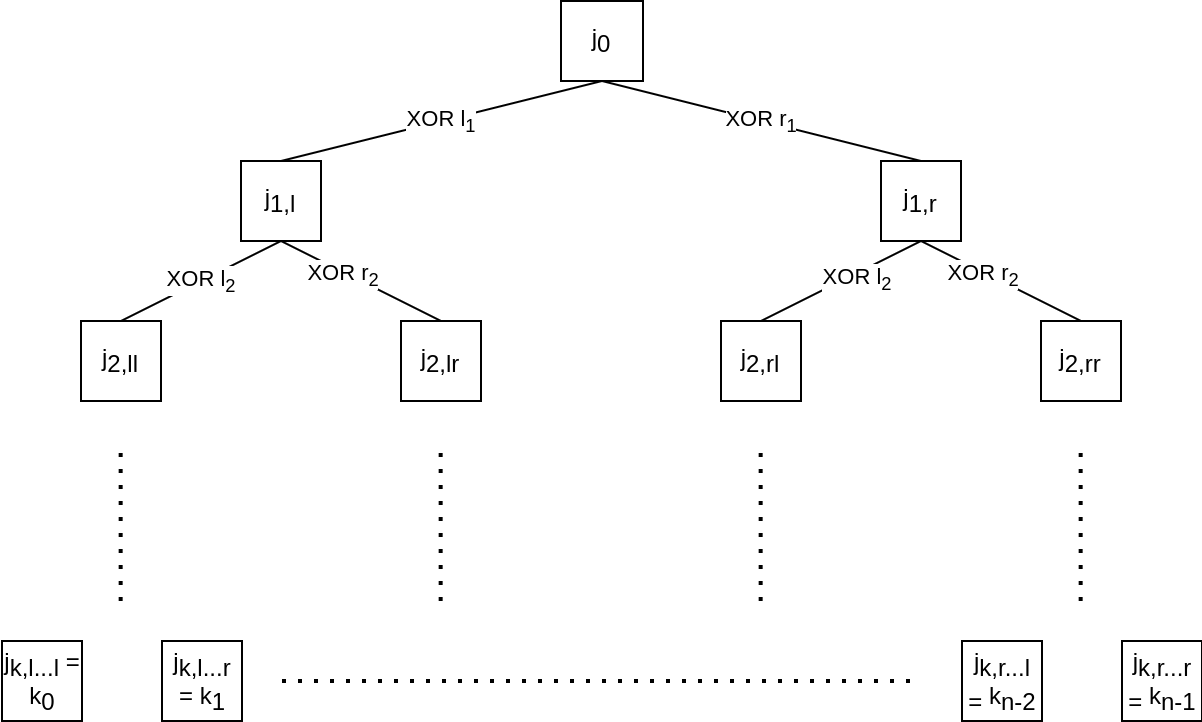
\includegraphics[width=\textwidth]{resources/key_generation}
		\caption{Key generation}
		\label{fig:keygen}
\end{figure}

Note that any $k_i$ is a random bit, being the result of an XOR operation with
random bits. Further any two $k_i, k_j$ with $i \neq j$ differ in at least one
of the XOR operations applied to $j_0$ to produce it. As all $l_i, r_i$
including the final $l_k, r_k$ are independently chosen, knowledge of any $k_i$
does not grant information about any $k_j, j \neq i$.

If we further associate each left edge with $0$ and each right edge with $1$,
then any $k_i$ can be found by following the sequence of edges corresponding to
the binary representation of $i$.

\subsection{n-1 OT}

Consider now the protocol in Algorithm \ref{alg:n_1_ot} for a
$\binom{n}{1}$-OT, where $n = 2^k$.

\begin{algo}
  \vbox{
    \small
    \begin{numbertabbing}
      xxxx\=xxxxxxxxxxxxxxxxxx\=xxxxxxxxxxxxx\=xxxxxxxx\=xxxxxxxxxxxxx\=xxxx\=MMMMMMMMMMMMMMMMMMM\=\kill
	  $S(x_0, \ldots, x_{n-1})$ \> \> \> \> \> $R(y)$ \\
	  \\
	  $j_0 = 0$ \> \> \> \> \> $k_y = 0$ \\
	  \> \> \> \> \> Binary representation of y \\
	  \> \> \> \> \> $(y_1 \ldots y_k)_2 := y$ \\
	  Key generation as shown in the previous section \\
	  \textbf{For} $i = 1$ to $k$ \\
	  \> $l_i \xleftarrow{R} \{0, 1\}$ \\
	  \> $r_i \xleftarrow{R} \{0, 1\}$ \\
	  \> $j_{i, x'l} = j_{i - 1, x'} \oplus l_i$ \\
	  \> $j_{i, x'r} = j_{i - 1, x'} \oplus r_i$ \\
	  $k_0, \ldots, k_{n-1} = j_{k, l \ldots l}, \ldots, j_{k, r \ldots r}$ \\
	  \\
	  $c_i = x_i \oplus k_i$ \> \> \> $\xrightarrow{c_0, \ldots, c_{n-1}}$ \\
	  \textbf{For} $i = 1$ to $k$ \> \> \> \> \> \textbf{For} $i = 1$ to $k$ \\
	  \> \> $\xrightarrow{l_i, r_i}$ \> $\binom{2}{1}$-OT \> $\xleftarrow{y_i}$ \\
	  \> \> \> \> $\xrightarrow{j_i}$ \> \> $k_y = k_y \oplus j_i$ \\
	  \> \> \> \> \> \textbf{Return} $c_y \oplus k_y$
    \end{numbertabbing}
  }
  \caption{$\binom{n}{1}$-OT using $k$ $\binom{2}{1}$-OT}
  \label{alg:n_1_ot}
\end{algo}

\subsubsection{Completness}

As noted earlier, each $k_i$ is found by following the edges (left edges being
$0$, right edges being $1$) corresponding to the binary representation of $i$.
As such $R$ will construct $k_y$ the same way $S$ did, and $c_y \oplus k_y =
x_y \oplus k_y \oplus k_y = x_y$.

\subsubsection{Security for S}

Due to the security of the $\binom{2}{1}$-OT, $R$ learns nothing about $k_z$
where $z \neq y$ Hence it also learns nothing about $m_z = c_z \oplus k_z$
where $z \neq y$.

\subsubsection{Security for R}

Due to the security of the $\binom{2}{1}$-OT, $S$ learns nothing about the bits
$y_i$ of $y$. As no other information is sent to $S$, it does not not learn of
the R's input $y$.

\subsection{Cost}

Assuming a $\binom{2}{1}$-OT implementation as shown in the lecture, this
protocol uses a total of:
\begin{itemize}
		\item $k$ $\binom{2}{1}$-OT, for a total of:
				\begin{itemize}
						\item $2k$ public-key operations
						\item $3k$ message rounds
						\item $O(k(1 + \lambda)) = O(k + k \lambda)$ bits
				\end{itemize}
		\item $2k$ random bits
		\item $2^{k+1} - 2$ XOR operations for key generation
		\item $2^k$ XOR operations for encryption
		\item $k$ XOR operations for key retrieval
		\item $1$ XOR operation for decryption
		\item $2^k = n$ bits and one message round for the transfer of the
				ciphertexts
\end{itemize}

Leading to a total cost of:
\begin{description}
		\item[Computational cost] $2k = 2 \log_{2}(n)$ expensive public-key
				operations and $O(n)$ cheap XOR operations
		\item[Latency] $3k + 1$ message rounds
		\item[Communication complexity] $O(n + k \lambda)$ bits transferred
\end{description}

\end{document}
